\chapter{Landau-Ginzburg Formalism}%TO DO!! fix the title

\noindent
The previous chapters developed the microscopic foundations of superconductivity: 
from the condensation of bosons in Bose--Einstein statistics to the pairing mechanism that gives rise to the Bardeen--Cooper--Schrieffer state. \\ 
We now turn to a complementary, macroscopic description capable of capturing the large-scale behaviour of superconductors without resolving their microscopic details.  
This is provided by the \emph{Landau--Ginzburg (LG) theory}, a phenomenological framework that expresses superconductivity through a complex order parameter~$\psi(\mathbf{r})$, interpreted as the macroscopic wavefunction of the condensate. Within this theory, spatial variations of~$\psi$ and electromagnetic fields are coupled through a free-energy functional, from which one derives the celebrated \emph{Ginzburg--Landau equations}. 

\section{Landau’s Theory of Phase Transitions}
\label{sec:landau_theory}

The thermodynamic classification of phase transitions introduced by \textit{Ehrenfest} distinguished first-- and second--order transitions according to discontinuities in the derivatives of the free energy.  
Although useful, this description was purely macroscopic and did not address the microscopic origin of the transition itself.  
\textit{Lev Landau} provided a deeper and more general description by linking second--order phase transitions to changes in the \textit{symmetry} of the physical system.

\subsection*{Spontaneous Symmetry Breaking in Ferromagnets}
To illustrate Landau’s reasoning, consider the case of a ferromagnet, whose behaviour is shown schematically in Fig.~\ref{Figure 6 - Ferro_vs_Para}.\\
At high temperatures $(T > T_c)$, the system is in the \emph{paramagnetic} phase: the atomic magnetic moments are randomly oriented due to thermal agitation, and the material as a whole exhibits no net magnetization. This corresponds to the \emph{high-symmetry} phase, where rotational symmetry is preserved.\\
As the temperature decreases below the Curie temperature $T_c$, the magnetic moments spontaneously align, giving rise to a finite magnetization M. The system thus selects a preferred direction in space, breaking the original rotational symmetry.\\
It is this spontaneous symmetry breaking, rather than a discontinuity in thermodynamic quantities, that, according to Landau, captures the true nature of a phase transition.

\begin{figure}[H]
    \centering
    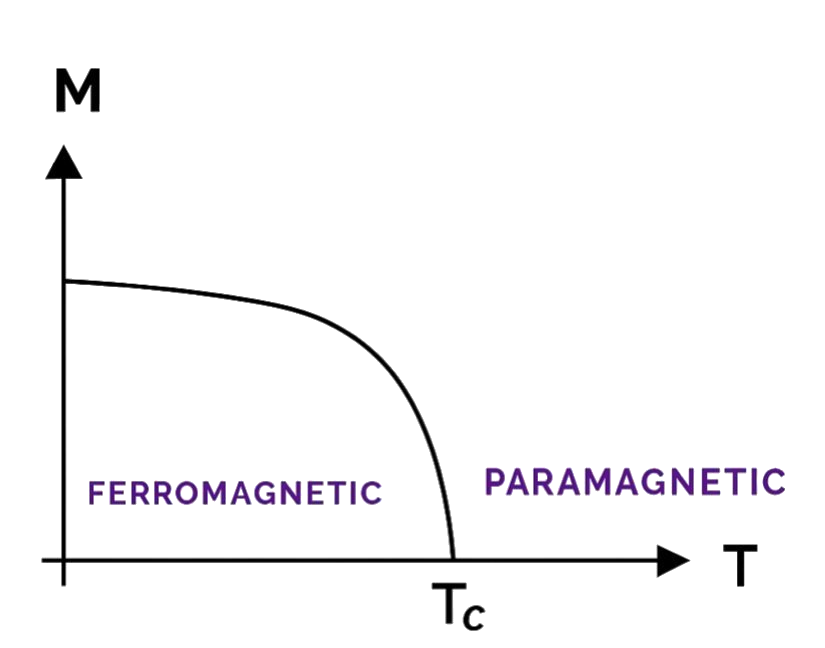
\includegraphics[scale= 0.5]{Chapters/Chapter_5/Images/6_ferromag2.png}
    \caption{Temperature dependence of the magnetization M in a ferromagnet.}
    \label{Figure 6 - Ferro_vs_Para}
\end{figure}

\subsection*{Free-Energy Expansion}
Landau’s key insight was that near the transition point, the state of the system can be described by an order parameter~$\eta$, which measures the degree of symmetry breaking.

\paragraph{The order parameter.}
The order parameter, denoted by \(\eta\), measures the degree of order in the system and distinguishes the two phases:
\[
\eta =
\begin{cases}
0, & T \geq T_c \quad \text{(symmetric phase)},\\[4pt]
\neq 0, & T < T_c \quad \text{(symmetry--broken phase)}.
\end{cases}
\]
For a ferromagnet, \(\eta\) corresponds to the magnetization \(M\); for a superconductor, it will later be identified with the complex condensate wavefunction \(\Psi(\mathbf{r})\).  
As the temperature crosses \(T_c\), the order parameter increases smoothly from zero to a finite value, signaling a continuous (second-order) phase transition.

\paragraph{Free-Energy Functional.}
The central assumption is that the \textit{free energy density} \(f\) of the system can be expanded as a power series in the order parameter \(\eta\), which is small near \(T_c\):
\begin{equation}
    f(T, \eta) = f_n(T) + a(T)\eta^2 + \frac{b(T)}{2}\eta^4 + \dots,
    \label{eq:landau_free_energy}
\end{equation}
where \(f_n(T)\) is the free energy of the normal (symmetric) phase and \(a(T)\), \(b(T)\) are phenomenological coefficients.  
The absence of odd powers in \(\eta\) reflects the assumption of symmetry between the two directions of the order parameter (\(\eta \leftrightarrow -\eta\)).  
The quartic term ensures stability since \(b(T) > 0\).

\paragraph{Equilibrium and Phase Behaviour.}
The equilibrium value of \(\eta\) minimizes the free energy:
\[
\frac{\partial f}{\partial \eta} = 0
\;\Rightarrow\;
2a(T)\eta + 2b(T)\eta^3 = 0.
\]
This yields two possible solutions:
\[
\eta = 0, \qquad \text{or} \qquad \eta^2 = -\frac{a(T)}{b(T)}.
\]
The first solution corresponds to the symmetric phase, the second to the symmetry--broken one.  
To determine which is stable, we examine the sign of \(a(T)\).  
Landau assumed that \(a(T)\) varies linearly near the critical temperature:
\[
a(T) = a_0 (T - T_c), \qquad a_0 > 0.
\]

Now:

\begin{itemize}
    \item For \(T > T_c\), the coefficient \(a(T) \) is positive. Then \(a(T)/b(T) > 0\), so the second solution \(\eta^2 = -a/b\) would be negative, i.e.\ unphysical (since \(|\eta|^2\) cannot be negative).  
    Hence, the only possible solution is
    \[
    \eta = 0.
    \]
    This means that the system minimizes its free energy when there is no order, the symmetric (normal) phase.

    \item For \(T < T_c\), the coefficient \(a(T) < 0\) is negative. Now \(-a/b > 0\), so the solution
    \[
    |\eta| = \sqrt{-\frac{a(T)}{b(T)}}
    \]
    is real and positive.  
    This implies that the free energy is minimized not at \(\eta = 0\), but at some finite value of \(|\eta|\).  
    The system spontaneously chooses one of the equivalent minima (e.g.\ \(+\eta\) or \(-\eta\)), thereby breaking the symmetry.
\end{itemize}

\begin{figure}[H]
    \centering
    %----------------------------------------
    % Panel 1: T > Tc (Single Minimum)
    %----------------------------------------
    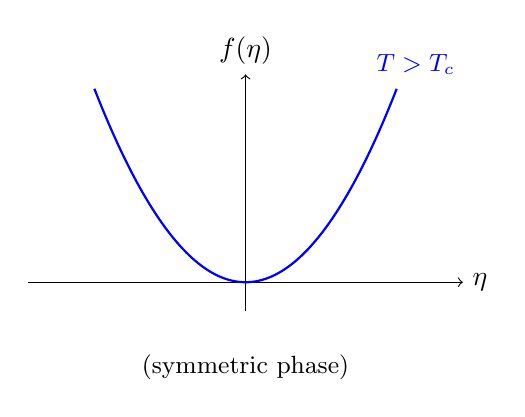
\begin{tikzpicture}[scale=1.2]
        % Axes
        \draw[->] (-2.3,0) -- (2.3,0) node[right] {$\eta$};
        \draw[->] (0,-0.3) -- (0,2.2) node[above] {$f(\eta)$};

        % Free energy curve: single well
        \draw[thick,blue,domain=-1.6:1.6,samples=100] 
            plot(\x,{0.8*\x*\x });
        
        % Label
        \node[above,blue] at (1.8,2.1) {\small $T > T_c$};
        \node at (0,-0.9) {\small (symmetric phase)};
    \end{tikzpicture}
    \hspace{1.5cm}
    %----------------------------------------
    % Panel 2: T < Tc (Double Well)
    %----------------------------------------
    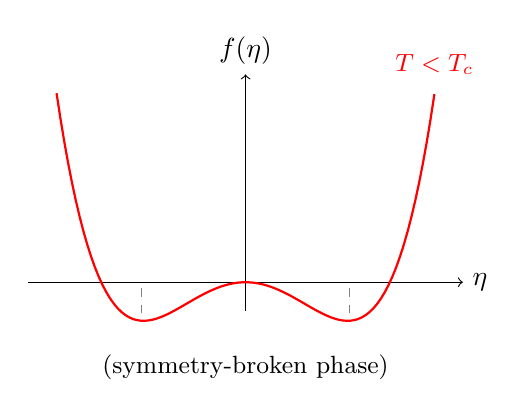
\begin{tikzpicture}[scale=1.2]
        % Axes
        \draw[->] (-2.3,0) -- (2.3,0) node[right] {$\eta$};
        \draw[->] (0,-0.3) -- (0,2.2) node[above] {$f(\eta)$};

        % Free energy curve: double well
        \draw[thick,red,domain=-2:2,samples=100] 
            plot(\x,{0.3*\x*\x*\x*\x - 0.7*\x*\x});

        % Dashed lines at minima
        \draw[dashed,gray] (-1.1,-0.33) -- (-1.1,0);
        \draw[dashed,gray] (1.1,-0.33) -- (1.1,0);
        %\node[below] at (-1.2,0.7) {\small $-\!|\eta|$};
        %\node[below] at (1,0.7) {\small $+|\eta|$};
        
        % Label
        \node[above,red] at (2,2.1) {\small $T < T_c$};
        \node at (0,-0.9) {\small (symmetry-broken phase)};
    \end{tikzpicture}

    %----------------------------------------
    % Caption
    %----------------------------------------
    \caption{
    Landau free energy $f(\eta)$ above and below the critical temperature $T_c$.  
    For $T > T_c$ (left), the free energy has a single minimum at $\eta = 0$, corresponding to the symmetric, normal phase.  
    For $T < T_c$ (right), $a(T)$ becomes negative and $f(\eta)$ develops two degenerate minima at $\pm|\eta|$, indicating spontaneous symmetry breaking and the emergence of long-range order.
    }
    \label{fig:landau_free_energy_panels}
\end{figure}

In the next section, we apply this phenomenological expansion to superconductivity by identifying the order parameter \(\eta\) with the complex macroscopic wavefunction \(\Psi(\mathbf{r})\), which represents the superconducting condensate.


\section{The Ginzburg--Landau Free Energy Functional}
\label{sec:GL-functional}

Having established Landau’s general framework for second-order phase transitions, 
we now apply the same reasoning to superconductivity.\\
In this context, the order parameter is the complex macroscopic wavefunction
\[
\Psi(\mathbf{r}) = |\Psi(\mathbf{r})| e^{i\phi(\mathbf{r})},
\]
which represents the collective quantum state of the superconducting condensate.\\
Following the Landau approach, the free energy of the superconducting phase is expanded in powers of the small quantity $|\Psi|$ near the critical temperature.

\subsection*{Free energy in the uniform case} 
Consider first a uniform superconductor in absence of external magnetic fields.  
Let $F_s(T,V)$ and $F_n(T,V)$ denote the free energies of the superconducting and normal states, respectively.\footnote{%
We use the \emph{free energy} rather than the internal energy because it depends naturally on temperature and is therefore suited for studying thermal phase transitions near $T_c$.}
Since the two phases differ just slightly close to $T_c$, the free energy of the superconducting phase can be written as
\begin{equation}
F_s(T,V) = F_n(T,V) + V\!\left[a(T)|\Psi|^2 + \frac{b(T)}{2}|\Psi|^4 + \dots\right],
\label{eq:GL_free_energy_uniform}
\end{equation}
where $a(T)$ and $b(T)$ are phenomenological coefficients, with $b(T) > 0$ ensuring stability. This is precisely the same form as the Landau expansion \eqref{eq:landau_free_energy}, now generalized to a complex order parameter.\\
The equilibrium value of $|\Psi|$ minimizes $F_s$.  
Neglecting higher-order terms, the condition $\partial F_s / \partial |\Psi| = 0$ gives
\[
|\Psi|^2 = 
\begin{cases}
0, & T > T_c,\\[4pt]
-\dfrac{a(T)}{b(T)}, & T < T_c,
\end{cases}
\qquad \text{with } a(T) = a_0(T - T_c), \ a_0 > 0.
\]
Thus, for $T > T_c$, the minimum occurs at $|\Psi| = 0$ (normal phase), 
whereas for $T < T_c$, the minimum appears at a finite $|\Psi|$, signaling the onset of superconductivity and the emergence of long-range order.


\begin{figure}[H]
    \centering
    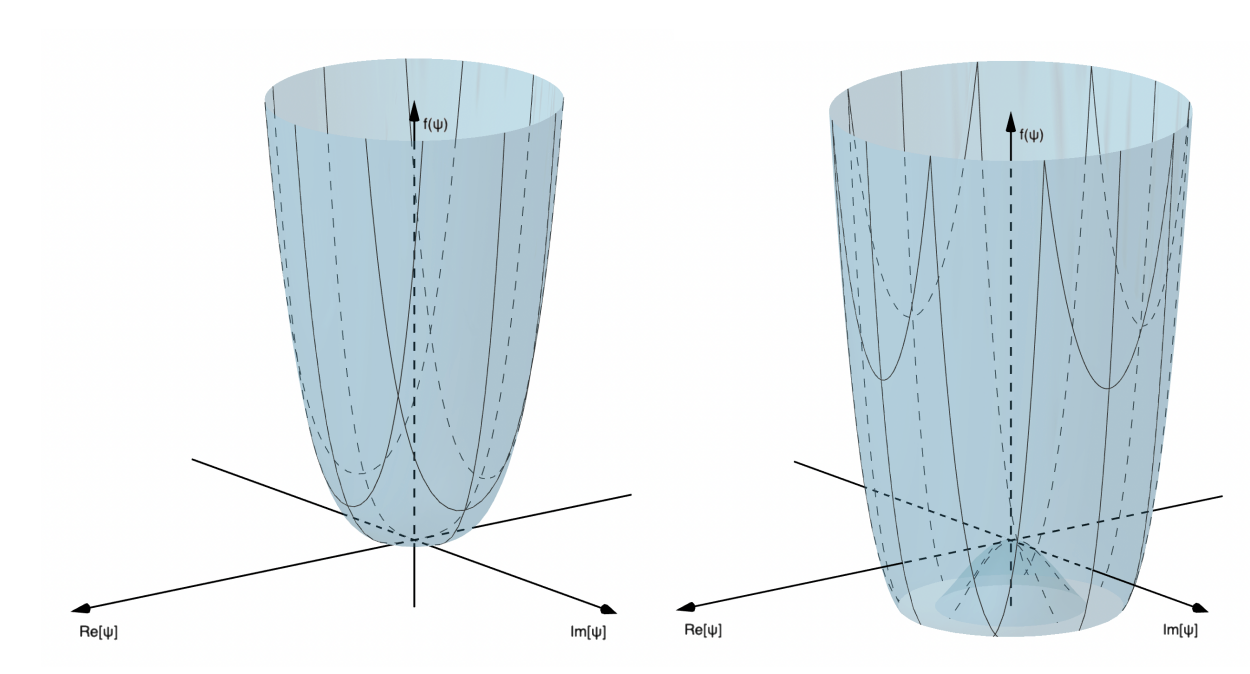
\includegraphics[scale = 0.6]{Chapters/Chapter_5/Images/7_mexican_hat.png}
    \caption{
    Complex order parameter $\Psi$. For $T > T_c$ (left), the potential has a single minimum at $\Psi = 0$, corresponding to the symmetric (normal) phase. For $T < T_c$ (right), the potential develops a continuous circle of degenerate minima at $|\Psi| = \sqrt{-a/b}$.
    }
    \label{fig:mexican_hat_GL}
\end{figure}

\subsection*{Inclusion of spatial variations and magnetic field}
In real materials, the order parameter is not uniform: its amplitude and phase can vary in space, particularly near surfaces, defects, or under the influence of magnetic fields.  
These spatial variations give rise to additional kinetic energy to the free energy, represented by a gradient term proportional to $|\nabla\Psi|^2$.  
Moreover, since the superconducting condensate carries charge, its momentum couples to the electromagnetic field through the \textit{minimal coupling} substitution\footnote{%
In principle, one could also include a scalar electric potential $\phi$ in the coupling, 
but for steady-state situations in a superconductor the perfect conductivity condition 
eliminates any static potential differences.  
Hence, $\phi$ can be neglected here.  
In dynamic situations, such as moving vortices, $\phi$ must be retained, 
but this lies beyond the static Ginzburg--Landau formulation considered in this chapter.%
}:
\[
\mathbf{p} \;\longrightarrow\; \mathbf{p} - q\mathbf{A},
\]
which corresponds to replacing the ordinary derivative by the \emph{gauge-covariant derivative}:
\[
\nabla \;\longrightarrow\; \nabla - i\frac{q}{\hbar}\mathbf{A},
\]
where $q = 2e$ is the charge of a Cooper pair and $\mathbf{A}$ is the magnetic vector potential.\\
Including these effects, the free energy functional becomes
\begin{equation}
F_s = F_n + \int d^3r
\left[
\frac{1}{2m^*}\bigl|(-i\hbar\nabla - q\mathbf{A})\Psi\bigr|^2
+ a(T)|\Psi|^2 + \frac{b(T)}{2}|\Psi|^4
\right],
\label{eq:GL_functional_noBfield}
\end{equation}
where $m^* = 2m_e$ is the effective mass of a Cooper pair.\\
The magnetic field itself also stores energy, given by the usual Maxwell term:
\[
\int d^3r\, \frac{|\mathbf{B}(\mathbf{r})|^2}{2\mu_0}
= \int d^3r\, \frac{(\nabla\times\mathbf{A})^2}{2\mu_0}.
\]
Adding this contribution yields the complete \emph{Ginzburg--Landau free energy functional}:
\begin{equation}
\boxed{
F_s = F_n + \int d^3r
\left\{
\frac{1}{2m^*}\bigl|(-i\hbar\nabla - q\mathbf{A})\Psi\bigr|^2
+ a(T)|\Psi|^2
+ \frac{b(T)}{2}|\Psi|^4
+ \frac{|\nabla\times\mathbf{A}|^2}{2\mu_0}
\right\}}\,.
\label{eq:GL_full_free_energy}
\end{equation}

Equation~\eqref{eq:GL_full_free_energy} describes the macroscopic behaviour of a superconductor through its order parameter and electromagnetic field.  
The first term represents the kinetic energy associated with spatial variations of the condensate, the next two describe the condensation energy, and the last term accounts for the magnetic-field energy.

Minimizing this functional with respect to $\Psi^*$ and $\mathbf{A}$ yields the coupled \emph{Ginzburg--Landau equations}, governing the spatial evolution of the superconducting order parameter and electromagnetic fields.

\section{The Ginzburg--Landau Equations}
\label{sec:GL_equations}

The Ginzburg--Landau free energy functional introduced in Eq.~\eqref{eq:GL_full_free_energy}
can be treated as a variational energy functional whose stationary configuration corresponds
to the equilibrium superconducting state.  
Minimizing it with respect to the complex conjugate of the order parameter $\Psi^*(\mathbf{r})$
and to the vector potential $\mathbf{A}(\mathbf{r})$ yields two coupled differential equations,
known as the \textit{Ginzburg--Landau equations}.

\subsection*{First Ginzburg--Landau equation}

The first equation follows from requiring that the free energy $F_s$ 
be stationary under infinitesimal variations of the complex order parameter.  
In this context, varying the functional with respect to $\Psi^*(\mathbf r)$ 
means determining how the free energy changes when the condensate wavefunction 
$\Psi(\mathbf r)$ and its conjugate $\Psi^*(\mathbf r)$ are independently perturbed.\\
Formally, the stationarity condition is expressed as\footnote{%
In variational problems involving complex fields, such as the superconducting order parameter, 
the field $\Psi$ and its complex conjugate $\Psi^*$ are treated as formally independent variables. 
Since the Ginzburg--Landau free energy $F_s[\Psi,\Psi^*]$ depends on both, one must require 
$\delta F_s/\delta\Psi = 0$ and $\delta F_s/\delta\Psi^* = 0$ for stationarity. 
These two conditions are complex conjugates of each other; 
it is customary to vary with respect to $\Psi^*$, which yields the equation of motion for $\Psi$.}:
\begin{equation}
\frac{\delta F_s}{\delta \Psi^*(\mathbf{r})} = 0,
\label{eq:GL_variation_Psi}
\end{equation}
ensuring that the free energy is stationary under small variations of $\Psi^*$.  
In analogy with classical variational principles, this condition defines the equilibrium configuration of the superconducting condensate.\\
Performing the functional derivative\footnote{%
For the full detailed derivation, see Appendix~\ref{app:GL-derivation}, 
Section~\ref{app:1_GL-derivation}.} 
of Eq.~\eqref{eq:GL_full_free_energy} gives
\begin{equation}
\boxed{
-\frac{\hbar^2}{2m^*}
\left(\nabla - i\frac{q}{\hbar}\mathbf{A}\right)^{\!2}\Psi(\mathbf{r})
+ a(T)\Psi(\mathbf{r})
+ b(T)|\Psi(\mathbf{r})|^2\Psi(\mathbf{r}) = 0.
}
\label{eq:first_GL_eq}
\end{equation}

This nonlinear equation governs the spatial behaviour of the superconducting order parameter 
in the presence of electromagnetic fields.  
The first term represents the kinetic energy associated with spatial variations of $\Psi$, 
the second describes the local condensation energy, and the cubic term 
$b(T)|\Psi|^2\Psi$ accounts for self-interaction between Cooper pairs.  
Together, they describe how both the amplitude and phase of the macroscopic 
wavefunction adjust to minimize the total free energy.

\subsection*{Supercurrent and the Second Ginzburg--Landau Equation}
The second equation follows from requiring the free energy to be stationary under infinitesimal variations of the vector potential~$\mathbf{A}(\mathbf{r})$.
The vector potential is not a fixed external field, it interacts with the superconducting condensate\footnote{%
The magnetic field depends on the current, and the current depends on the magnetic field.}, and the two must be determined self-consistently.
To understand how the magnetic field behaves inside the material, we examine how the free energy changes when $\mathbf A$ is varied.

The free energy depends on the vector potential $\mathbf A$ in two ways:
through the magnetic-field energy term $(|\nabla\times\mathbf A|^2)$, and through its coupling to the superconducting condensate $(|(-i\hbar\nabla - q\mathbf A)\Psi|^2)$.
If $\mathbf A$ changes, both the magnetic field and the kinetic energy of the condensate change, thereby modifying the total free energy of the system.\\
To describe this response quantitatively, we introduce the supercurrent density $\mathbf{J}_s$, defined as the functional derivative of the free energy with respect to $\mathbf A$:
\begin{equation}
\mathbf{J}_s(\mathbf r) = -\,\frac{\delta F_s}{\delta \mathbf A(\mathbf r)}.
\label{eq:Js_variational_def_main}
\end{equation}
Physically, this means that $\mathbf{J}_s$ measures how the system reacts when the magnetic field (or equivalently $\mathbf A$) is varied.
The supercurrent acts as the source of the magnetic field inside the superconductor, and the two quantities influence one another: changing the magnetic field changes the current, and vice versa.\\
A small variation of $\mathbf A$ therefore produces a corresponding change in free energy,
\[
\delta F_s = -\!\int \mathbf J_s \cdot \delta\mathbf A\, d^3r,
\]

\paragraph{Expression for the supercurrent.}
Evaluating the derivative\footnote{%
For the full detailed derivation, see Appendix~\ref{app:GL-derivation}, 
Section~\ref{app:2_GL-derivation}.} in Eq.~\eqref{eq:Js_variational_def_main} for the GL functional gives
\begin{equation}
\boxed{
\mathbf{J}_s =
\frac{i q \hbar}{2 m^*}\bigl(\Psi\,\nabla\Psi^* - \Psi^*\,\nabla\Psi\bigr)
- \frac{q^2}{m^*}|\Psi|^2\mathbf{A}.
}
\label{eq:Js_expression_main}
\end{equation}
The first term arises from gradients in the phase of $\Psi$,
while the second represents the coupling of the condensate to the electromagnetic potential $\mathbf A$.

\paragraph{Phase representation and superfluid velocity.}
Expressing $\Psi = |\Psi| e^{i\theta}$, with $|\Psi|$ constant, makes the structure of the current transparent:
\[
\mathbf{J}_s
= \frac{q\hbar}{m^*}\,|\Psi|^2
\left(\nabla\theta - \frac{q}{\hbar}\mathbf A\right).
\]
The term in parentheses is a gauge-invariant momentum per unit $\hbar$, 
which vanishes when the local phase gradient compensates the electromagnetic potential.  
It is natural to define from it the \emph{superfluid velocity} of the Cooper pairs:
\begin{equation}
\mathbf v_s = \frac{\hbar}{m^*}
\left(\nabla\theta - \frac{q}{\hbar}\mathbf A\right),
\end{equation}
so that $\mathbf J_s = q\,|\Psi|^2\,\mathbf v_s$
takes the same form as the current density of a charged fluid with density $|\Psi|^2$ and charge $q$.
The vector $\mathbf v_s$ therefore describes the collective motion of the condensate,
and spatial variations of the phase $\theta(\mathbf r)$ correspond to macroscopic supercurrents.

\paragraph{Second Ginzburg--Landau equation.}
The magnetic field obeys Ampère’s law,
\[
\nabla\times\mathbf B = \mu_0(\mathbf J_s + \mathbf J_{\rm ext}),
\qquad \mathbf B = \nabla\times\mathbf A,
\]
and substituting Eq.~\eqref{eq:Js_expression_main} gives
\begin{equation}
\boxed{
\nabla \times (\nabla \times \mathbf{A})
= \mu_0
\left[
\frac{i q \hbar}{2 m^*}
\bigl(\Psi\,\nabla\Psi^* - \Psi^*\,\nabla\Psi\bigr)
- \frac{q^2}{m^*}|\Psi|^2\mathbf{A}
+ \mathbf{J}_{\text{ext}}
\right].
}
\label{eq:second_GL_eq_main}
\end{equation}

\bigskip
Together, Eqs.~\eqref{eq:first_GL_eq} and~\eqref{eq:second_GL_eq_main}
form a closed system describing the self-consistent interaction 
between the superconducting condensate and the electromagnetic field.

A vital outcome of these equations is the determination of two intrinsic material length scales: the coherence length ($\xi$) and the magnetic penetration depth ($\lambda$). The ratio of these two lengths, known as the Ginzburg--Landau parameter ($\kappa = \lambda / \xi$), acts as a single, decisive parameter. This dimensionless parameter $\kappa$ determines the fundamental way a superconductor responds to an applied magnetic field and is used to gather different behaviours, leading to the classification of superconducting materials into two distinct groups: \textbf{Type I and Type II superconductors}.


%\subsection{Empirical determination of GL parameters}

\section{Magnetic Penetration Depth and Coherence \\Length}

Before discussing the classification of superconductors, it is useful to introduce
two intrinsic characteristic lengths that naturally arise within the
Ginzburg–Landau theory:
\begin{itemize}
    \item the \textbf{magnetic penetration depth}~$\lambda$, which measures how far
    magnetic fields can penetrate into a superconductor before being screened by
    supercurrents;
    \item the \textbf{coherence length}~$\xi$, which characterizes the typical
    distance over which the order parameter $\Psi$ can vary spatially.
\end{itemize}
These two fundamental scales describe the balance between magnetic and
condensate energies in the superconducting state.  
Their ratio,
\begin{equation}
\kappa = \frac{\lambda}{\xi},
\end{equation}
known as the \textit{Ginzburg--Landau parameter}, plays a decisive role in determining
the magnetic response of a superconductor.  
In the following subsections, we derive explicit expressions for $\lambda$ and $\xi$,
which will later allow us to distinguish between Type~I and Type~II superconductors.


\subsection*{Magnetic Penetration Depth $\lambda$}
\label{sec:penetration_depth}

The first intrinsic length scale obtained from the Ginzburg–Landau theory is the
\textit{magnetic penetration depth}~$\lambda$. This parameter measures how far a magnetic field can penetrate into a superconductor before being exponentially screened by supercurrents, and we will show that it is equivalent to the \textit{London penetration depth} $\lambda_L$ introduced in Section \ref{Lond_eq}.

\paragraph{London limit.}
Let us start from the general expression for the supercurrent density:
\[
\mathbf{J}_s =
\frac{i q \hbar}{2 m^*}
\bigl(\Psi\,\nabla\Psi^* - \Psi^*\,\nabla\Psi\bigr)
- \frac{q^2}{m^*}|\Psi|^2\mathbf{A}.
\]
In the case of a uniform condensate (the so-called London limit, where spatial variations of $|\Psi|$ are negligible), the amplitude $|\Psi|$ is constant. Furthermore, in a situation where the phase is uniform ($\nabla\theta = 0$), the superflow contribution (the first term, related to the gradient of the phase) vanishes. The current density then reduces to the simple form:
\begin{equation}
\mathbf{J}_s = -\,\frac{q^2}{m^*}\,|\Psi|^2\,\mathbf{A}.
\label{eq:london_current_GL}
\end{equation}
This expression corresponds exactly to the microscopic form of the \textit{first London equation}\footnote{%
Originally derived in Section~\ref{Lond_eq}, Eq.~\eqref{000}.},
here obtained directly from the Ginzburg--Landau order parameter~$\Psi$.

\paragraph{Derivation.}
By substituting this GL-derived London current [Eq.~\eqref{eq:london_current_GL}] into Ampère’s law ($\nabla\times\mathbf{B} = \mu_0\,\mathbf{J}_s$), the resulting differential equation for the magnetic field $\mathbf{B}$ is mathematically identical to the London differential equation derived in Section \ref{Lond_eq}:
\begin{equation}
\nabla^2\mathbf{B}
= \frac{1}{\lambda^2}\,\mathbf{B}.
\label{eq:GL_london_equation}
\end{equation}
This confirms that the magnetic field decays exponentially ($\mathbf{B}(x) \propto e^{-x/\lambda}$) over the characteristic length $\lambda$, which is defined by the parameters of the Ginzburg-Landau order parameter:
\begin{equation}
\boxed{
\lambda^2 = \frac{m^*}{\mu_0 q^2 |\Psi|^2}.
}
\label{eq:penetration_depth_GL}
\end{equation}
This result demonstrates the consistency between the Ginzburg–Landau and London descriptions, identifying $\lambda$ with the London penetration depth $\lambda_L$.

\subsection*{Coherence Length}
The coherence length $\xi$ follows from the linearized form of the first Ginzburg–Landau equation in absence of magnetic fields ($\mathbf A=0$), where the order parameter $\Psi$ is small, typically near the critical temperature $T_c$. This length scale characterizes the distance over which $\Psi$ can vary spatially within the superconductor.

\paragraph{Derivation.}

In the zero field case ($\mathbf A=0$), the first GL equation reads
\[
-\frac{\hbar^2}{2m^*}\,\nabla^2 \Psi + a(T)\,\Psi + b(T)\,|\Psi|^2\Psi = 0.
\]
Close to $T_c$ the order parameter is small, so the cubic term can be neglected, giving the linearized equation
\[
-\frac{\hbar^2}{2m^*}\,\nabla^2 \Psi + a(T)\,\Psi \simeq 0
\quad\Longrightarrow\quad
\nabla^2 \Psi = \frac{2m^*\,a(T)}{\hbar^2}\,\Psi.
\]
For $T<T_c$ one has $a(T)<0$, and spatial deviations of $\Psi$ relax exponentially. Defining the characteristic length $\xi$ by
\[
\nabla^2 \Psi = -\frac{1}{\xi^2}\,\Psi,
\]
and using $|a(T)|=-a(T)$ below $T_c$, one obtains
\begin{equation}
\frac{1}{\xi^2}=\frac{2m^*\,|a(T)|}{\hbar^2}
\quad\Longrightarrow\quad
\boxed{\;\xi(T)=\sqrt{\frac{\hbar^2}{2m^*\,|a(T)|}}\, .\;}
\end{equation}

\section{Type I and Type II Superconductors}
\label{sec:type_I_II}

Superconductors can be classified into two fundamental categories, \textit{Type I} and \textit{Type II}, according to their magnetic behaviour in an external field.\\
This distinction arises naturally from the Ginzburg–Landau theory, through the dimensionless parameter
\[
\kappa = \frac{\lambda}{\xi}.
\]
The parameter $\kappa$ represents the relative balance between magnetic and condensation energies:
it compares the characteristic distance over which magnetic fields are screened ($\lambda$) 
with the distance over which the order parameter recovers its bulk value ($\xi$).  

\begin{itemize}
  \item For $\kappa < 1/\sqrt{2}$, the energy cost of forming a normal–superconducting boundary is \emph{positive}, and magnetic flux is completely expelled until the superconducting state abruptly collapses at a single critical field $H_c$.  
  Materials of this kind are called \textbf{Type I superconductors}.
  \item For $\kappa > 1/\sqrt{2}$, the interface energy becomes \emph{negative}, and the system favours the penetration of magnetic flux in the form of quantized vortices.  
  These materials are called \textbf{Type II superconductors}.
\end{itemize}

Thus, $\kappa = 1/\sqrt{2}$ defines the boundary between the two regimes.  
The difference in magnetic behaviour between Type~I and Type~II superconductors follows directly from this energetic balance and is reflected in their magnetization response, shown in Fig.~\ref{fig:typeI_typeII_magnetization}.  

\begin{figure}[H]
\centering
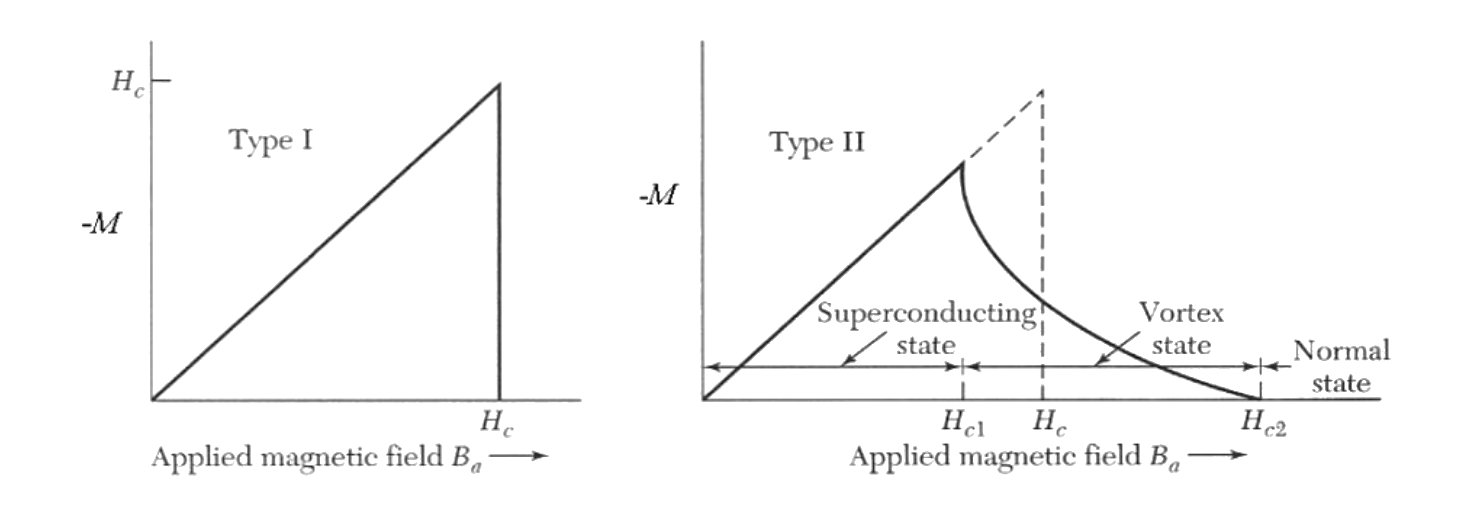
\includegraphics[scale=0.6]{Chapters/Chapter_5/Images/4_type1_type2_2.png}
\caption{
Magnetization curves for Type~I (left) and Type~II (right) superconductors.
Adapted from \cite{raes2021}.
}
\label{fig:typeI_typeII_magnetization}
\end{figure}

In Type~I superconductors, the magnetic field is completely expelled up to the critical field $H_c$, where superconductivity collapses abruptly.  
In Type~II materials, magnetic flux penetrates progressively between two critical fields, $H_{c1}$ and $H_{c2}$, giving rise to an intermediate \textit{mixed state} where normal and superconducting regions coexist, as illustrated in Fig.~\ref{fig:typeI_typeII_magnetizatic_field}.

\begin{figure}[H]
\centering
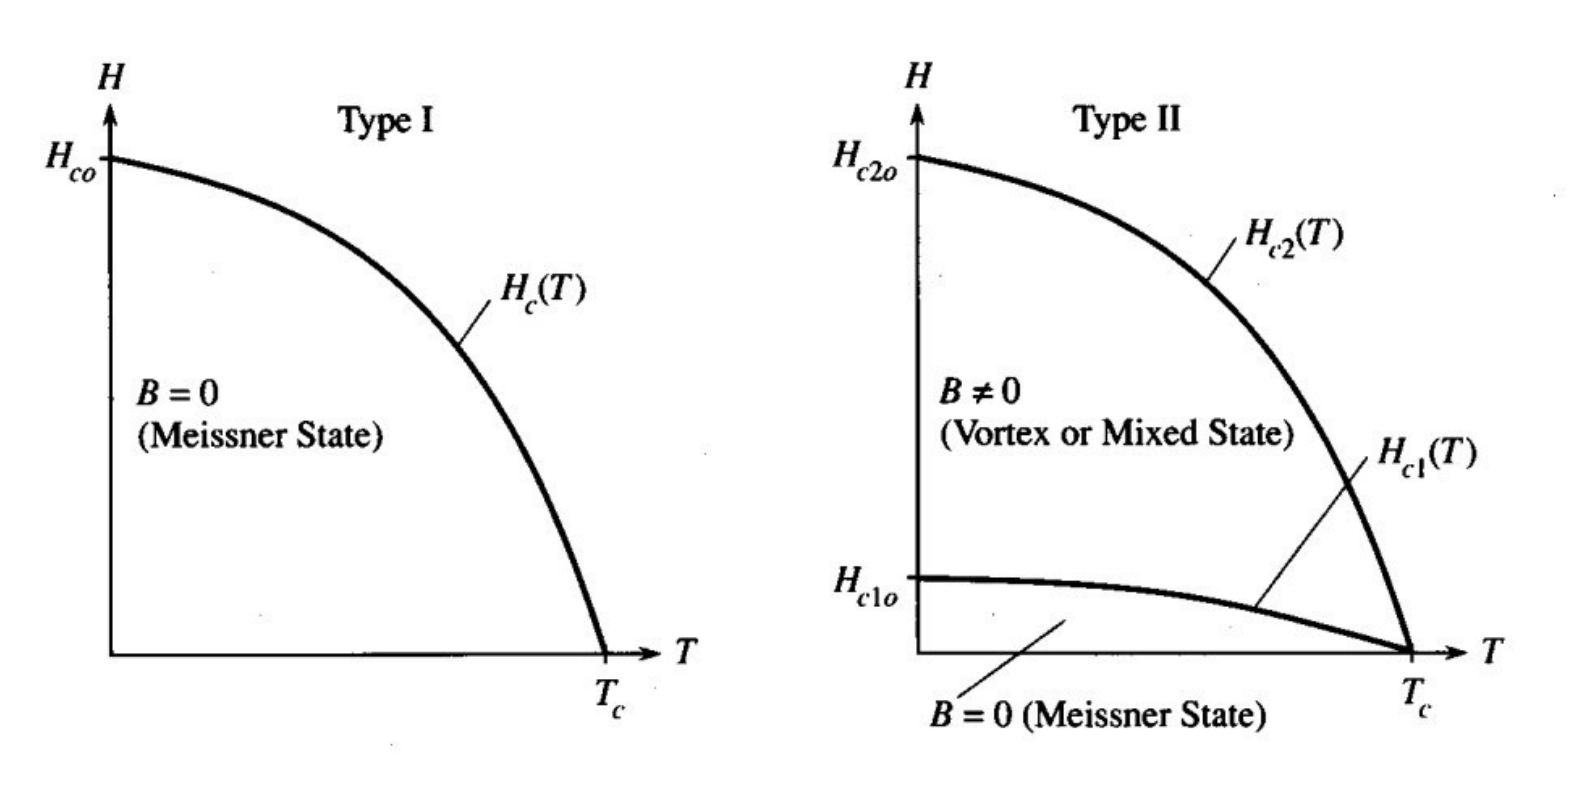
\includegraphics[scale=0.45]{Chapters/Chapter_5/Images/5_states.png}
\caption{
Schematic illustration of magnetic field penetration in Type~I and Type~II superconductors.  
Type~I materials exhibit complete flux expulsion up to $H_c$, while in Type~II materials quantized flux lines penetrate between $H_{c1}$ and $H_{c2}$, forming the mixed (vortex) state.  \\
Image adapted from \cite{raes2021}.
}
\label{fig:typeI_typeII_magnetizatic_field}
\end{figure}

\subsection*{Type I Superconductors}

Type I superconductors are characterized by complete magnetic flux expulsion up to a single critical magnetic field $H_c$.  
For applied fields $H < H_c$, the material remains entirely in the superconducting state, exhibiting perfect diamagnetism ($\mathbf{B}=0$ in the bulk) as a manifestation of the Meissner effect.  
When the field reaches $H_c$, the superconducting state collapses abruptly, and the material transitions uniformly to the normal state.

From an energetic perspective, the interface between a superconducting region and a normal one involves two opposing contributions:
\begin{enumerate}
    \item the \textit{condensation energy gain} $\varepsilon_C$, associated with the formation of the superconducting state, extending over a distance $\xi$;
    \item the \textit{magnetic energy cost} $\varepsilon_B$, associated with expelling the magnetic field, extending over the penetration depth $\lambda$.
\end{enumerate}
In Type I superconductors ($\xi > \lambda$), the magnetic energy cost dominates, leading to a \textit{positive surface energy}. The system thus avoids forming interfaces, preferring to remain either entirely superconducting or entirely normal.  
This explains the single critical field and the absence of partial flux penetration.

\begin{figure}[H]
\centering
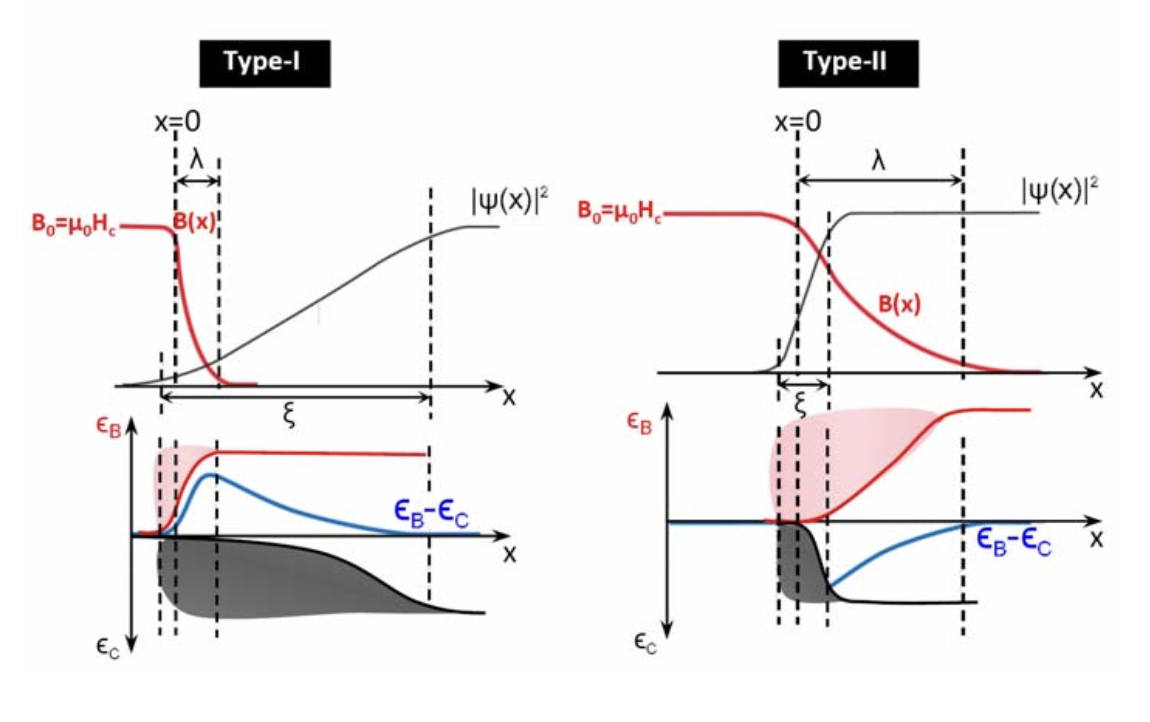
\includegraphics[scale = 0.8]{Chapters/Chapter_5/Images/1_type_1_2.png}
\caption{
Magnetic field (red), order parameter $|\Psi(x)|^2$ (black), and interfacial energy balance for Type I (left) and Type II (right) superconductors.
In Type I materials ($\xi > \lambda$), the interface energy is positive: magnetic flux is completely expelled until the superconducting state collapses at $H_c$.\\
Image adapted from \cite{raes2021}.
}
\label{fig:typeI_typeII_interface}
\end{figure}

The top panels of Fig.~\ref{fig:typeI_typeII_interface} illustrate how, in a Type I material, the magnetic field decays over $\lambda$ while the order parameter recovers over $\xi$.  
The bottom panels show the corresponding energy densities: in the Type I case, the magnetic energy $\varepsilon_B$ exceeds the condensation energy $\varepsilon_C$, making $\varepsilon_B - \varepsilon_C > 0$, i.e.\ interface formation is energetically unfavourable.

Experimentally, Type I superconductors show a sharp transition in their magnetization curve at $H_c$.  
Below $H_c$, the magnetization decreases linearly with the applied field ($\mathbf{B}=0$), whereas above $H_c$ superconductivity is destroyed and $\mathbf{B}=\mu\mathbf{H}$, as shown in Fig.~\ref{fig:typeI_typeII_magnetization}.  
This behaviour is typical of elemental metals such as Pb, Hg, Sn, and Al, which exhibit low critical fields (tens of mT) and critical temperatures below $7$~K.

\subsection*{Type II Superconductors}

Type II superconductors exhibit a richer magnetic behaviour due to their negative interface energy ($\lambda > \xi$).  
At low fields, they behave identically to Type I materials: magnetic flux is completely expelled, and the Meissner effect is preserved.  
However, as the applied field increases, the energetic balance at the boundary between the normal and superconducting regions changes.  
In this case, the magnetic energy gained by allowing partial field penetration over a distance $\lambda$ exceeds the condensation energy cost associated with suppressing the order parameter over $\xi$ (see Fig.~\ref{fig:typeI_typeII_interface}).  
The total surface energy therefore becomes negative, so that the formation of normal–superconducting interfaces lowers the total free energy.  
The system thus finds it energetically favourable to let magnetic flux enter locally, forming many small normal regions embedded in a superconducting matrix.  

\paragraph{Vortices and the Abrikosov lattice.}
When the applied magnetic field exceeds a first critical value $H_{c1}$, magnetic flux begins to penetrate the material in discrete, quantized filaments known as \textit{vortices}.  
These vortices correspond to tiny cylindrical regions where the superconducting order parameter $\Psi$ vanishes and the magnetic field is locally concentrated.  
Between the lower and upper critical fields, $H_{c1}$ and $H_{c2}$, the superconductor enters the so-called \textit{mixed state}, in which normal and superconducting regions coexist.  


\begin{figure}[H]
\centering
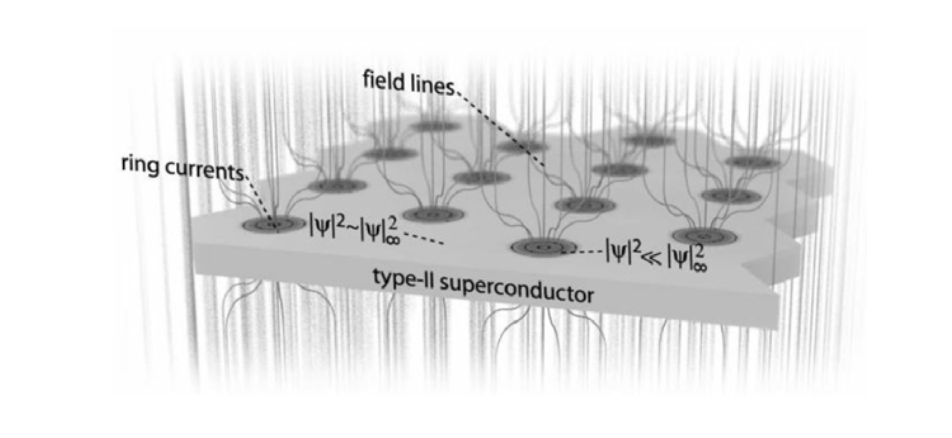
\includegraphics[scale = 0.72]{Chapters/Chapter_5/Images/3_abrikosov.png}
\caption{
An Abrikosov lattice of vortices in a Type~II superconductor.\\
Image adapted from \cite{moshchalkov2011}.
}
\label{fig:abrikosov_lattice}
\end{figure}
As the field increases, the vortices interact repulsively and arrange themselves into a regular, periodic pattern, the \textit{Abrikosov lattice}, which minimizes the total free energy by balancing magnetic and condensation energies.
This ordered structure is characteristic of Type~II superconductivity and is illustrated in Fig.~\ref{fig:abrikosov_lattice}.  \\
As the applied field approaches $H_{c2}$, the density of vortices grows until their cores overlap, at which point superconductivity is completely destroyed and the material becomes normal.\\
Each vortex carries one quantum of magnetic flux,
\begin{equation}
\Phi_0 = \frac{h}{2e},
\end{equation}
and is surrounded by circulating supercurrents that decay over the London penetration depth~$\lambda$.  
The detailed internal structure of a single vortex is shown in Fig.~\ref{fig:vortex_structure}: the magnetic field $B(r)$ peaks at the vortex centre, where $|\Psi|^2$ vanishes, and both quantities recover their bulk values over a characteristic distance $\xi$.

\begin{figure}[H]
\centering
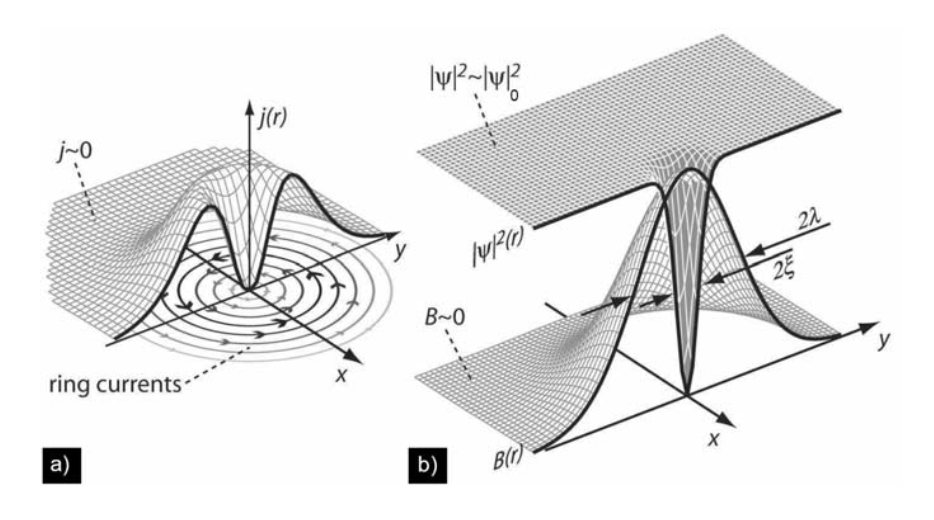
\includegraphics[scale = 0.8]{Chapters/Chapter_5/Images/2_vortex.png}
\caption{
Spatial structure of a single vortex in a Type~II superconductor.  
(a) The supercurrent density forms circular loops around the vortex core and decays on the length scale $\lambda$.  
(b) The order parameter $|\Psi|^2$ vanishes at the vortex centre and recovers over $\xi$, while the magnetic field $B(r)$ peaks in the core and decays outward.  \\
Image adapted from \cite{raes2021}.
}
\label{fig:vortex_structure}
\end{figure}

Type~II superconductors include metallic alloys (NbTi, Nb$_3$Sn) and high-temperature cuprates (YBa$_2$Cu$_3$O$_{7-x}$), which maintain superconductivity under extremely high magnetic fields, up to several tens of tesla, making them essential for technological applications such as particle accelerators.

To highlight the main differences in material properties and critical parameters, 
Table~\ref{tab:typeI_typeII_materials} summarizes representative examples of both Type~I and Type~II superconductors.

\begin{table}[H]
\centering
\renewcommand{\arraystretch}{1.2}
\setlength{\tabcolsep}{5pt}
\small
\begin{tabular}{lccc|lcc}
\hline
\multicolumn{3}{c|}{\textbf{Type I Superconductors}} & 
\multicolumn{3}{c}{\textbf{Type II Superconductors}} \\[2pt]
\textbf{Material} & $T_c$ [K] & $H_c$ [mT] &
\textbf{Material} & $T_c$ [K] & $H_{c2}$ [T] \\ 
\hline
Aluminium (Al)     & 1.2  & 10   & Niobium (Nb)          & 9.3   & 0.4  \\
Tin (Sn)           & 3.7  & 30   & Nb--Titanium (NbTi)   & 9.2   & 14   \\
Lead (Pb)          & 7.2  & 80   & Nb--Tin (Nb$_3$Sn)    & 18    & 25   \\
Mercury (Hg)       & 4.2  & 41   & Vanadium (V)          & 5.3   & 0.9  \\
Zinc (Zn)          & 0.9  & 5    & YBa$_2$Cu$_3$O$_{7-x}$ (YBCO) & 92 & $>100$ \\
\hline
\end{tabular}
\caption{
Representative examples of Type~I and Type~II superconductors with typical critical parameters. 
}
\label{tab:typeI_typeII_materials}
\end{table}


\subsection*{The Emergence of Type III Superconductors}
Beyond the conventional dichotomy of Type~I and Type~II superconductors, recent theoretical developments and experimental observations have revealed superconducting behaviours that do not fit neatly within this traditional classification.
In particular, certain materials display magnetic and transport characteristics that cannot be fully explained by the standard Ginzburg–Landau framework or by the simple $\kappa$-based criterion distinguishing the two known types.

To account for these unconventional phenomena, the concept of a \textbf{Type~III superconductor} has been introduced. These materials exhibit several distinctive physical characteristics that set them apart from conventional superconductors:

\begin{itemize}
    \item \textbf{Inhomogeneous structure:} Type III materials consist of microscopic superconducting regions (or ``droplets'') separated by non-superconducting or weakly superconducting barriers.  
    Their macroscopic superconducting properties emerge from the collective coupling of these regions, rather than from a uniform condensate.
    \item \textbf{Beyond Ginzburg–Landau theory:}  
    The behaviour of these systems cannot be fully captured within the conventional Ginzburg–Landau formalism. Their superconducting properties arise from collective and spatially nonuniform effects that lie beyond the assumptions of a continuous, homogeneous order parameter.
    \item \textbf{Coreless vortices:} In contrast to the \textbf{Abrikosov vortices} of Type II superconductors, which possess a normal (non-superconducting) core of size $\xi$, the vortices in Type III materials are predicted to be \textbf{coreless} (Josephson vortices).  
    These arise in weakly coupled granular or layered systems, where superconducting phase coherence persists without a normal core.
    \item \textbf{Dissipationless transport:} Because these vortices lack a normal core, their motion does not produce resistive dissipation.  
    This feature enables \textbf{lossless current flow} even in the presence of strong magnetic fields, offering potential advantages over conventional Type II superconductors in high-field applications.
\end{itemize}

The emergence of Type III superconductivity thus extends the traditional classification of superconductors, highlighting how material granularity, multi-component order parameters, and topological effects can lead to qualitatively new superconducting phases.  
